\chapter{Local Control: Obeying Constraints}

\graphicspath{{control_constraints/images/}}

\section{INTRODUCTION}
% Motivation
Manipulation of deformable objects is essential for many applications, such as surgery, doing laundry, and industrial assembly. 
However, robotic manipulation of deformable objects remains a challenging problem. One of the central difficulties is modeling and predicting the state of the object.
%make sure we say we only do objects like cloth and rope (no volume preservation)
The compliant nature of objects like cloth and rope (we do not consider volume-preserving or elastic objects in this work) entails that their motion depend on a large set of physical properties. To model and predict the state of the deformable object, most previous work focuses on constructing a precise physical model, e.g., using Mass-Spring \cite{Essahbi2012} or Finite-Element \cite{Muller2002} models. 
We seek to create a controller for practical deformable object manipulation tasks that does not rely on detailed knowledge of physical properties, i.e. that does not have a highly-accurate physical model. 
Such models require parameters (both physical and numerical) that are difficult to obtain and are usually more time-consuming to compute, preventing their use in a fast control loop. 





Controlling objects such as cloth or rope is made more difficult by the fact that they have an infinite number of degrees of freedom. The system, which consists of a set of grippers which hold the deformable object, is also extremely underactuated. %(e.g. an object  are extremeThe high number of degrees of freedom of these objects makes sensing, control, and planning even more difficult \cite{Polygon_Skeleton}.
On top of this, it is also challenging to design a practical controller for manipulation that preserves constraints, such as the avoidance of overstretching of the object, due to a lack of direct control of deformation.  
% mention the draw-back in previous work in exact modeling
%The primary limitation of these methods include high dimensionality, difficulty in parameters tuning, and their performance is susceptible to discretization. 

%make sure it is clear what we mean by not doing simulation and how that is different from much previous work
%\textcolor{red}{These models aim to approach the object motion by doing a highly accurate physical simulation, where they explicitly study the elemental-wise effects on the object based on the physical law.


The model in this paper will not involve precise physical simulation. Instead, we aim to construct an approximate model that predicts the object motion based on geometric information, such as the current poses of the grippers and the current configuration of the deformable object. Previous work on this kind of modeling \cite{Berenson2013} approached the problem by exploiting a property called \textit{diminishing rigidity}, which assumes that the effect of gripper motion along the deformable object diminishes as the distance from the gripper increases. 
This method has shown that it is possible to do practical manipulation tasks with a deformable object without a precise physical model. 
However, we observe that this rigidity does not only diminish as the distance from the gripper increases. Instead, it is a function of a larger set of variables derived from the configuration of the object. The rigidity also depends on the direction of gripper motion. Fig.\ref{Fig: intro_Directional_rigidity} shows an example of an object's directional rigidity.

\begin{figure}[t]
\begin{subfigure}{.26\textwidth}
  \centering
  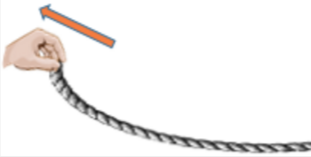
\includegraphics[width=.75\linewidth]{Intro_drag}
%  \caption{}
  \label{Fig: Intro_drag}
\end{subfigure}%
\begin{subfigure}{.24\textwidth}
  \centering
  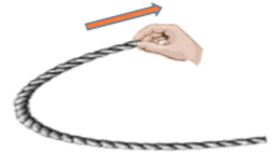
\includegraphics[width=.75\linewidth]{Intro_pull}
%  \caption{}
  \label{Fig: Intro_pull}
\end{subfigure}
\caption{An illustrative example of directional rigidity. Left: The rope moves almost rigidly when dragging it by one end to the left. Right: The rope deforms when pulling it on the right in the opposite direction.}
\label{Fig: intro_Directional_rigidity}
\end{figure}


%% Controller and constraints
%Some controllers are designed with a physical model to represent the deformable object \cite{Dmitry_cite_14} \cite{Dmitry_cite_15}. 
%However, these controllers rely on an explicit model to represent the deformable object and do not consider obstacle avoidance or compensation for excessive stretching. 
%For obstacle avoidance, \cite{Berenson2013} and \cite{Dmitry_cite_18} make use of the null-space of the Jacobian to allow movements that do not interfere with the obstacle avoidance constraint.
%To mitigate the excessive stretching, %\cite{Berenson2013} and \cite{Dale_Bandit} attempt to compensate for the excessive stretching by correcting the desired object motion sent to the controller. 
%The effect of such corrections is extremely limited due to the compliant nature of the deformable object. 
%Instead, our approach is to prevent the excessive stretching by setting constraints in the controller.%to the robot operation space.

%% Explain the key contribution, specify the directional rigidity and constraint violation in introduction
% Brief outline of the structure of the rest of the paper.
Thus the key contributions of this paper are:
1) A geometric model for deformable object manipulation that is computationally efficient to use in a control loop while capturing the directional rigidity effects more accurately than that in \cite{Berenson2013}; and
%2) A method that enforces that model predictions do not penetrate into obstacles by projecting points to the obstacleA prediction of the object movement improves the accuracy of the controller compared to that of \cite{Berenson2013} by addressing the directional rigidity during the object motion and the non-penetrating obstacle constraints on the object. 
2) A controller that addresses the excessive stretching constraint by better approximating which directions of motion lead to more/less stretching. This new constraint is especially important when the object is caught on an obstacle, which the method in \cite{Berenson2013} does not address.




Since we build on the idea described in \cite{Berenson2013}, we use this method as a benchmark in our experiments. 
We compared \cite{Berenson2013} with our proposed method in several simulation and physical robot experiments. We found that the proposed model is able to predict the object motion better than the previous model and that the new controller is more effective at preventing overstretch than the method in \cite{Berenson2013}.
%\todo{Revise this paragraph for the real-robot experiment}

In the remainder of the paper, we discuss related work and present the problem statement. We then describe our new model formulation and how to formulate the constraints for the controller. Finally, we describe the results of running this method in several test scenarios.


\section{RELATED WORK}

%\todo{ Cite the papers mentioned by Reviewer 3 for both the "On sensing/estimation of deformation" and the "On deformation control:"}

Deformable object manipulation has been studied in many contexts ranging across domestic, surgical, and industrial domains \cite{Jimenez2012}. Much of this work relies on accurate modeling and simulation of deformable objects. Some of the most common simulation methods use Mass-Spring Models \cite{Essahbi2012, Maris2010} and Finite-Element Models (FEM) \cite{Muller2002}, However, such approaches usually require significant tuning and are very sensitive to discretization parameters. Also, we seek a model that can be evaluated very quickly inside an optimal control framework, and Finite-element models, while accurate, can be computationally-expensive to simulate. While methods have been developed to track objects using FEM in real-time \cite{Petit2017}, a controller may need to evaluate the model many times to find an appropriate command, requiring speeds faster than real-time. Specialized models have also been developed, e.g., \cite{Borum2014} and \cite{Bretl2014} focus on elastic rods that are not in contact. We seek a model that works well with rope- and cloth-like materials that can deform as a result of contact. Finally, researchers have also investigated automatic modeling of deformable objects \cite{Lang2002, Cretu2008}. However, these methods rely on a time-consuming training phase for each object to be modeled, which we would like to avoid.%and it requires a lot of efforts in preparing test cases.

Given a model such as those above, researchers have investigated various control methods to manipulate deformable objects. %Some controllers are designed with an explicit model to represent the deformable object. 
Hirai and Wada proposes an iterative visual-servoing controller in \cite{Hirai2000}, which aligns interest points on the deformable object to targets. 
Its control law is based on modeling the deformable object as a lattice of interconnected springs. 
\cite{Wada2001} uses a similar spring model to formulate a PID controller that aligns interest points to targets. While effective, these methods rely on models like those above and thus suffer from the above issues.
%All these controllers rely on an explicit model to represent the deformable object which can induce the high computation cost and heavy parameters tuning work.


Our work is complementary to methods that adapt the model of the object during manipulation \cite{Navarro-Alarcon2014, NavarroAlarcon2018, Hu2018deformable_gpr}. Our model can serve as an initial guess and a reference for such methods so that the online adaptation process does not diverge too far from a reasonable model as a result of perception or modeling error. 
%However these models require a good initial guess of the Jacobian to begin the adaptation process. The work proposed here could serve as such a guess. %Instead of an exact model of the deformable object, they explore the features of the dynamics from the task space. 
%The philosophy of the deformable object modeling in this paper is very close to these works. 
Our paper builds on the idea of diminishing rigidity Jacobians \cite{Berenson2013} by improving the model and formulating appropriate constraints for deformable object manipulation. \cite{McConachie2018} extended \cite{Berenson2013} to use multiple Jacobian-based models when it is uncertain which model is appropriate for the object. The new model proposed here could be incorporated into the framework of \cite{McConachie2018}. 
%and study the methods to tune the Jacobian-based model, as well as the way to maximize the rewards of tasks by selecting the right controller for operation.


% manipulation model in the B.M
The model and controller in this paper are built on the method for deformable object manipulation in \cite{Berenson2013} and task space control of robot manipulators \cite{Khatib1987}.
However, unlike \cite{Berenson2013}, we explore the directional diminishing rigidity of the deformable object. This maintains a low computational cost of prediction while improving accuracy.
%Our approach to handling obstacle avoidance is similar to \cite{Berenson2013} and \cite{Sentis2005} in that it repels the gripper from obstacles using the surface normal. As a result, the prediction of object movements will not interfere with the obstacle avoidance constraint.

% over-stretching constraint in other controller and the B.M
Much previous work in this area focuses on completing a task but does not consider constraints on obstacle avoidance or compensation for excessive stretching \cite{Hirai2000, Wada2001}. \cite{Berenson2013} does consider these constraints but its stretching-avoidance method does not handle cases where the object is caught on an obstacle because it does not reason about the way strain propagates through the object as a result of gripper motion. We consider this issue in our paper.

%the correction for excessive stretching is assigned as a point-wise correction on the deformable object. The controller then applies the inverse of the non-explicit prediction model on this correction term to get the resulting correction term as robot motion.  
%This method has limit achievement in correcting the stretching term due to the highly-inaccurate non-explicit model and the lack of control on the most region on the object by the robot. 
%In this paper, we consider the lack of control on the object and define a stretching vector for each robot gripper and use it to mitigate the stretching avoidance constraint in robot configuration space.






\section{PROBLEM STATEMENT}
\label{sec:problemstatement}
Let a set of $P$ points $\mathcal{P}\subset \mathbb{R}^{3P}$ be the configuration of the deformable object, where these points are either in the curve of a 1D object (e.g., rope) or on the surface of the 2D object (e.g., cloth). 
%\todo{"not mention 3D object", should clarify that we only deal with 1D and 2D objects}
This paper focuses on 1D and 2D objects like cloth and rope. We do not consider volume-preserving or elastic objects.
Denote the object velocity as $\dot{\mathcal{P}} = [\dot{p}_1^T,..., \dot{p}_P^T]^T \in \mathbb{R}^{3P}$.
Let $q\in SE(3)^G$ be the configuration of a set of $G$ grippers. 
%Let the function $\mathcal{F}: \mathbb{Q} \rightarrow \mathbb{R}^{3P}$ be the mapping from the grippers configuration $q$ to the position of the points in the deformable object $\mathcal{P}$. 
Denote the velocity of the robot to be $\dot{q} = [\dot{q}_1^T, ... \dot{q}_G^T]^T$ and the velocity of the $g$th gripper $\dot{q}_g = [v_g^T \ \omega_g^T]^T \in \mathfrak{se}(3)^G$, 
where $\mathfrak{se}(3)$ is the tangent space of $SE(3)$ \cite{Murray1994}, 
$v_g$ is the translation components, and $\omega_g$ is the rotation components. 

%Let $\phi $: $\mathfrak{se}(3)^G \rightarrow \mathbb{R}^{3P}$ 
Let $\phi$ be the mapping such that $\dot{\mathcal{P}} = \phi (q,\dot{q},\mathcal{P},\mathcal{O})$, where $\mathcal{O}$ denotes the configurations of obstacles in the environment and $\mathcal{P}$ is the object configuration at the current state.
Let $C_c$ denote the set of gripper motions $\dot{q}$ which preserve the gripper collision constraint and $C_s$ denote the set of $\dot{q}$ which preserve the object stretching constraint.

In this paper we assume that the grippers are free-floating and we have a method of sensing $\mathcal{P}$. 
%\todo{ “we assume that …… we have a method of sensing P.” Is it a practical assumption and how about the computational efficiency and real-time performance of tracking P?}
Inverse-kinematics can be used to track these gripper motions with robot arms. 
%\todo{"Why is it Inverse-kinematics"}
We do not consider stretching as a result of friction, as friction forces are negligible when compared with the stretching induced by the robot pulling on the object for the tasks we consider.
%Furthermore, we neglect the object stretching resulting from the friction and consider the stretching arising from pairs of the grippers motions interacting with each other.

Overall, our goal is to move the $G$ grippers such that the motion of points in $\mathcal{P}$ best matches commanded motions $\dot{\mathcal{P}}_d$, without violating constraints. To achieve this, we must address two fundamental problems: 1) Design an approximate model $\tilde{\phi}$ which is practical to be used by the robot controller with improved accuracy compared to the benchmark \cite{Berenson2013}. 2) Prevent robot collision and excessive stretching of the object by specifying a set of constraints $C = C_c\cap C_s$. We formalize this control problem as a constrained optimization problem: 

%The optimizer we use to solve the problem is NOMAD \cite{Nomadsolver}, a black-box nonlinear optimization solver.

\begin{equation}
\begin{aligned}
& \underset{\dot{q}}{\text{minimize}}
& & ||\dot{\mathcal{P}}_{d} - \tilde{\phi} (q, \dot{q},\mathcal{P},\mathcal{O})|| \\
& \text{subject to}
& & \dot{q} \in C, \\ 
& & &||\dot{q}||\Delta t < \Delta_{q,\textrm{max}}.
\end{aligned}
\label{Eq: Optimization Problem}
\end{equation}

%\todo{How to address the optimization algorithm used?}

\section{METHODS}
%\todo{"should have an explicit subsection to address the directional rigidity of material", "Section IV is quite difficult to read", " the clarity of how the parameters for directional rigidity are to be identified in use" }

To fully specify the problem in Eq. \ref{Eq: Optimization Problem}, we need to construct the approximate model $\tilde{\phi}$ and define the set of constraints $C$.  A highly accurate model for object motion can require a high computational cost when using FEM simulation. To make a model practical to be used by a robot controller with lower computational cost, we build on the idea of constructing a geometry-based model \cite{Berenson2013}. 

To create a more accurate model, we need to improve the accuracy of the $\tilde{\phi}$ approximated in \cite{Berenson2013} by capturing more accurate behavior of the object and addressing contact with the environment.
To that end, we design a model accounting for directional rigidity and obstacle-penetration constraints (Section \ref{Method_Jacobian-based Model of Deformable Object Motion}). We then define the collision avoidance constraint $C_c$ and object over-stretching constraint $C_s$ in the robot's task space (Section \ref{Method_Constraint Preserving Controller}).

%Specifically, the collision avoidance is addressed by checking the distance between each gripper and its nearest obstacle given the robot motion $\dot{q}$, 
%and the stretching avoidance is addressed by checking the alignment of the $\dot{q}$ with a set of stretching vectors. The stretching vectors are defined by tracking the relative positions of each gripper to a specific set of its neighboring points on the object.

%In this section, \textcolor{red}{\ref{Method_Jacobian-based Model of Deformable Object Motion}} will introduce the Jacobian-based model for improving the accuracy of the controller. \textcolor{red}{\ref{Method_Constraint Preserving Controller}} will discuss the methods of formulating the constraints. \todo{use labels and references instead of explicitly writing section numbers}

\subsection{Geometric Model of Deformable Object Motion} \label{Method_Jacobian-based Model of Deformable Object Motion}

\subsubsection{Model Overview}
The approximate model locally describes the object's motion when given a motion of the grippers. Below we describe our approach first by specifying the model and then enforcing collision constraints on the prediction this model makes.

The current state of the deformable object is a function of the current gripper pose, the history of gripper motions that have been applied, the object's initial configuration, and the obstacles in the environment:

\begin{equation}
    \mathcal{P} = F(q, Q_{hist},\mathcal{P}_0,\mathcal{O})
\end{equation}

To create a predictive model, we need to compute how $\mathcal{P}$ changes as a result of changing the gripper pose. Taking the time derivative of the above we obtain

\begin{equation}
\frac{\partial \mathcal{P}}{\partial t} = \frac{\partial F}{\partial q} \frac{\partial q}{\partial t} + \frac{\partial F}{\partial Q_{hist} } \frac{\partial Q_{hist}}{\partial t}+\frac{\partial F}{\partial \mathcal{P}_0} \frac{\partial \mathcal{P}_0}{\partial t} +\frac{\partial F}{\partial \mathcal{O}} \frac{\partial \mathcal{O}}{\partial t} \end{equation}

\noindent Only the first term is non-zero, thus

\begin{equation}
    \dot{\mathcal{P}} = \frac{\partial F(q, Q_{hist},\mathcal{P}_0,\mathcal{O})}{\partial q} \dot{q}%= %\frac{\partial F(q,\mathcal{P},\mathcal{O})}{\partial q}
\end{equation}

$\frac{\partial F}{\partial q}$ is a matrix we call $J$. In previous work \cite{Berenson2013}, $J$ is assumed to be independent of $\dot{q}$ and $\mathcal{O}$, yielding\footnote{In this equation we replaced $Q_{hist}$ and $\mathcal{P}_0$ with $\mathcal{P}$, the current configuration of the object. $Q_{hist}$ and $\mathcal{P}_0$ are need in $F$ to compute the current state of the object, but if we can sense $\mathcal{P}$ directly (as we assume), then $Q_{hist}$ and $\mathcal{P}_0$ are not needed to compute $J$.} $\frac{\partial F}{\partial q} = J(q,Q_{hist},\mathcal{P}_0) = J(q,\mathcal{P})$, which is analogous to a rigid-body Jacobian. While these assumptions allow a linear relationship between $\dot{q}$ and $\dot{\mathcal{P}}$, and thus computational convenience, they are not accurate in many situations (see Figure \ref{Fig: intro_Directional_rigidity} for an example). In this paper we change the definition of $J$ to the following:

\begin{equation}
    \dot{\mathcal{P}} = J(q,\dot{q},\mathcal{P},\mathcal{O})\dot{q} = \tilde{\phi}(q,\dot{q},\mathcal{P},\mathcal{O})
\end{equation}

We now describe how $J$ is computed, focusing on how it accounts for directional rigidity (using $\dot{q}$) and how it enforces obstacle penetration constraints (using $\mathcal{O}$).


\subsubsection{Directional Rigidity}
We build on the idea proposed in \cite{Berenson2013}, which approximates $J$ based on the observation that the deformable object behaves rigidly near points grasped by the robot grippers. \cite{Berenson2013} encoded this effect through a simple function that only considered the distance of a point from the the nearest gripper. However, we find that we can exploit geometric information in the object's configuration to better predict the object's motion when we use a more complex model. We have observed that the key features of the deformable object configuration for predicting its motion are its deformability (which is determined by its material properties) and where it is slack.  
%These features impair the transmission of motion from end to end, and make the dynamics different from the rigid ones.  
The deformation influences the transmission of the force from the grippers, i.e. the more stretchable the object, the more it will stretch when force is applied. However, when a region of the object is taut, regardless of how stretchable it is, it will move as if it were rigidly connected to a gripper (e.g. imagine a rope held taut by two grippers). %Whether or not the object is taut depends of course on the previous motion of the robot and the current configuration of this object. 
We also must take into account that points are not influenced equally by different grippers, i.e. grippers farther away contribute less to the motion of a point than those closer to it.


To incorporate the above effects into our model, we define the following variables, which can be derived from $q, \dot{q}$, and $\mathcal{P}$:
\begin{itemize}
    \item $\rho_{ij}$: the geodesic distance (a scalar) between points $p_i$ and $p_j$ on the surface of the object.
    \item $d_{ij}$: the vector starting at a point $p_i$ and ending at the point $p_j$, as shown in Fig. \ref{Fig: method_direction_rigidity}
    \item $q_g$: the configuration of the $g$th gripper
    \item $\dot{q}_g$: the velocity of the $g$th gripper.
\end{itemize}

Furthermore, let $c(i,g)$ be the index of the point with the minimal geodesic distance to $p_i$ among the ones grasped by the $g$th gripper. 
We address the notion of rigidity in object motion by considering the slackness of the object and reformulating the rigidity as a function of $\rho_{ic(i,g)}$, $d_{ic(i,g)}$, 
and $\dot{q}_g$. For each point $p_i$ we compute
\begin{equation}
\begin{split}
J^{dr}(q_g, \dot{q}_g, p_i)     &=\\
                   \theta_{i,g} &[w_{t,i,g} J^{dr}_{t}(q_g, \dot{q}_g, p_i), w_{r,i,g} J^{dr}_{r}(q_g, \dot{q}_g, p_i)] \\
w_{t,i,g}                       &= w_{t}(\rho_{ic(i,g)}, d_{ic(i,g)}, \dot{q}_g) \\    
w_{r,i,g}                       &= w_{r}(\rho_{ic(i,g)}) \\
J^{dr}_{t}(q_g, \dot{q}_g, p_i) &= \mathcal{I}_{3\times 3} \\
J^{dr}_{r}(q_g, \dot{q}_g, p_i) &= [R_g[1] \times r, R_g[2] \times r, R_g[3] \times r]
\end{split}
\label{Eq: trans_rot_rigidity_diminishing_jacobian}
\end{equation}
%\todo{I split the definitions of the w functions out, make sure it is correct}
%\todo{"the notation of Rg[n] is different with others."}
where $R_g[n]$ is the $n$th column of the rotation matrix of the $g$th gripper at the current configuration, $r = p_{c(i,g)} - v_g$, with $v_g$ being the translation of the $g$th gripper.
$w_{t,i,g}$ and $w_{r,i,g}$ are the corresponding translational and rotational diminishing rigidity factors defined by the point $p_i$ and $g$th gripper (discussed below). 

Our goal is to encode the directional rigidity of the object motion into $w_{t,i,g}$ and $w_{r,i,g}$ and use $\theta_{i,g}$ to describe the \textit{influence} of gripper $g$ on $p_i$. Intuitively, $w_{r,i,g}$ should decrease with the increasing geodesic $\rho_{ic(i,g)}$ distance between $p_i$ and $p_{c(i,g)}$. This is because the deformation of the region between $p_i$ and $p_{c(i,g)}$ will attenuate the transmitted force of the gripper's motion unless the object is taut. % the transmission of this movement.
Since the effects on $w_{r,i,g}$ from $\dot{q}_g$ and $d_{i,c(i,g)}$ are not as clear or significant as $\rho_{ic(i,g)}$, we keep the $w_{r,i,g}$ as a function of $\rho_{ic(i,g)}$, where 

\begin{enumerate}
    \item $w_{r,i,g}$ ranges between $0$ and $1$.
    \item $w_{r,i,g}$ decreases as $\rho_{ic(i,g)}$ increases.
\end{enumerate}
\noindent We give the definition of $w_{r,i,g}$ below.

From observation, we find two key reasons related to the slackness of the object that induce the diminishing rigidity effect for translation motion, and we aim to encode these factors into $w_{t,i,g}$. 
The first case is that the moving direction of $\dot{q}_g$ makes the region on the object between $p_i$ and $p_{c(i,g)}$ less taut.
The second case is that this region is already slack.
$w_{t,i,g}$ is thus a product of two terms:
\begin{equation}
w_{t,i,g} = \alpha_{i,g} \cdot \beta_{i,g}
\label{Eq: Combined_directional_rigidity}
\end{equation}
where $\alpha_{i,g}$ addresses the effect in the first case (motion reducing tension),
and $\beta_{i,g}$ addresses the effect in the second case (object slackness). 
Both $\alpha_{i,g}$ and $\beta_{i,g}$ are functions of some of $q_g, \dot{q}_g, p_i$, or variables derived from these.

For $p_i$ on the object, we find $\alpha_{i,g}$ is greatly impacted by $d_{ic(i,g)}$ and $\dot{q}_{ic(i,g)}$.
Decomposing $\dot{q}_g$ into $\dot{q}_{g,r}$, the radial component in the direction of $d_{ic(i,g)}$, and $\dot{q}_{g,t}$, the transverse component perpendicular to $d_{ic(i,g)}$. 
We observed that if $\dot{q}_{g,r}$ is in the opposite direction to $d_{ic(i,g)}$, then it is more likely to make the intervening region slacker and thus reduce the transmission of force from the gripper to $p_i$.
Moreover, if $\dot{q}_{g,r}$ and $d_{ic(i,g)}$ are in the same direction when the object is not already slack, $p_i$ can move almost rigidly with $\dot{q}_g$. 
Fig.\ref{Fig: intro_Directional_rigidity} shows an example of the impact of this alignment.      
Based on these observations, we design the function $\alpha_{i,g}=\alpha (d_{ic(i,g)},\dot{q}_g)$ with the following properties:
\begin{enumerate}
\item $\alpha (d_{ic(i,g)},\dot{q}_g)$ ranges between $0$ and $1$.
% \item $\alpha (d_{ic(i,g)},\dot{q}_g)= 1$ if $\langle d_{ic(i,g)},\dot{q}_g \rangle > 0$.
\item $\alpha (d_{ic(i,g)},\dot{q}_g) > \alpha (d_{jc(j,g)},\dot{q}_g)$ if \\ 
$\langle d_{ic(i,g)},\dot{q}_g \rangle > \langle d_{jc(j,g)},\dot{q}_g \rangle$ and \\ 
$\rho_{ic(i,g)} = \rho_{ic(i,k)}$.
\item $\alpha (d_{ic(i,g)},\dot{q}_g) > \alpha (d_{jc(j,g)},\dot{q}_g)$ if \\ 
$\langle d_{ic(i,g)},\dot{q}_g \rangle = \langle d_{jc(j,g)},\dot{q}_g \rangle$ and \\
$\rho_{ic(i,g)} > \rho_{ic(i,k)}$.
\end{enumerate}
We give the definition of $\alpha (d_{ic(i,g)},\dot{q}_g)$ below.


As mentioned above, $\beta_{i,g}$ depends on the current slackness of the intervening region. 
Without other external forces applied on the object, the pulling force applied by the robot will tend to unwind or unfold the object eventually (we do not consider cases where the object is tied into knots).  
For this reason,  the part of the intervening region on the object that is not already spread out is less likely to move rigidly with the $g$th gripper. 
One indicator that can address this property is the ratio between the Euclidean distance between $p_i$ and $p_{c(i,g)}$, and the geodesic distance $\rho_{ic(i,g)}$ between them. 
We denote $\mathfrak{r}_{i,g} = \frac{||d_{ic(i,g)}||}{\rho_{ic(i,g)}}$ to be this ratio.
A larger $\mathfrak{r}_{i,g}$ indicates a tauter intervening region. 
A tauter intervening region is more likely to result in $\dot{p}_i$ moving more rigidly.
Thus we can design the function $\beta_{i,g} = \beta (\mathfrak{r}_{i,g})$ with the following properties:%, where $\mathfrak{r}_{i,g}$ is the indicator derived from $d_{ic(i,g)}$ and $\rho_{ic(i,g)}$.
\begin{enumerate}
\item $\beta (\mathfrak{r}_{i,g})$ ranges between $0$ and $1$.
\item $\beta (\mathfrak{r}_{i,g})= 1$ if $\mathfrak{r}_{i,g} = 1$.
\item $\beta (\mathfrak{r}_{i,g}) > \beta (\mathfrak{r}_{i,g})$ if $\mathfrak{r}_{i,g} > \mathfrak{r}_{i,g}$
\end{enumerate}

Finally, $\theta_{i,g}$, which captures the influence of gripper $g$ on point $p_i$ should have the following property (where $k$ is the index of a different gripper on the robot):
\begin{enumerate}
\item $\theta_{i,g}$ ranges between $0$ and $1$.
\item $\theta_{i,g} < \theta_{i,k}$ if $\rho_{ic(i,g)} > \rho_{ic(i,k)}$.
\item $\sum_{m = 0}^{G} \theta_{i,m} = 1$.
\end{enumerate}


Through experimentation, we obtained good results with the following functions:
\begin{equation}
\begin{split}
\alpha & = e^{k_g \rho_{ic(i,g)}(\cos \angle(d_{i,c(i,g), \dot{q}_g}) -1)}  \\
%\alpha (d_{ic(i,g)},\dot{q}_g) & =
%e^{k_g(\langle d_{ic(i,g)},\dot{q}_g \rangle -|\langle d_{ic(i,g)},\dot{q}_g \rangle |)} \\
\beta (\mathfrak{r}_{i,g}) & = \left( \frac{||d_{ic(i,g)}||}{\rho_{ic(i,g)}} \right) ^{k_D} \\
w_{r}(\rho_{ic(i,g)}) & = e^{-k_{r}\rho_{ic(i,g)}} \\
\theta_{i,g} & = \frac{x_g}{\sum_{m = 0}^G x_m}\\
x_m & = \frac{\textrm{min} \{\rho_{ic(i,1)}, ... , \rho_{ic(i,G)}\}}{\rho_m} 
%\frac{\rho_{\textrm{min}}}{\rho_m}  \\
%\textcolor{red}{\rho_{\textrm{min}}} & = \textrm{min} \{\rho_{1c(i,1)}, ... , \rho_{Gc(i,G)}\} 
\end{split}
\label{Eq: functions_in_this_paper}
\end{equation}

% \todo{make sure diminishing rigidity k is mentioned here and parameter value is given in the results}


%\todo{" The used functions are dependent on parameters ('$k_g$', '$k_d$', '$k_r$'), these seem to be dependent on the type of material/object, how straightforward is to estimate these for a new object? "}
\noindent where $k_g$, $k_D$, and $k_{r}$ are non-negative parameters. Specifically, a larger $k_g$ indicates a greater impact on the diminishing in the rigidity from the motion reducing tension. A larger $k_D$ indicates a greater impact on the diminishing in the rigidity from the slackness of the object in the current state. 
A larger $k_{r}$ indicates a faster decrease in the rigidity of $J^{dr}_{r}$ as the distance from $p_i$ to the gripper increases. 


%\todo{"the geodesic distance is on top of the rope (orange line) could be made clearer by using a dashed red line, or make the orange line a bit thicker."}
\begin{figure}[t]
  \centering
  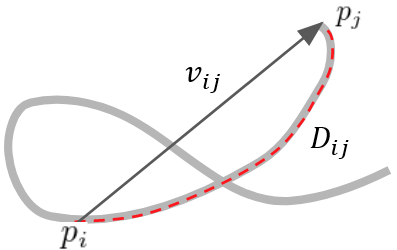
\includegraphics[width=1.5in]{method_geodesic.png}
  \caption{The length of the the red segment on the rope is the geodesic distance $\rho_{ij}$. $d_{ij}$ is the vector showing the relative position of $p_j$ with respect to $p_i$.}
  \label{Fig: method_direction_rigidity}
\end{figure}

\subsubsection{Obstacle Penetration Constraints}
%\subsubsection{Prediction of object motion when in contact with obstacles}
With the model developed above, we get a prediction of a point's movement from $\tilde{\dot{p}}_i = J^{dr}(q_g, \dot{q}_g, p_i)\dot{q}$. 
However, at this stage, we haven't take into account the effect from the obstacles $\mathcal{O}$. Thus the predicted $\tilde{\dot{p}}_i$ can move $p_i$ into an obstacle.

When the prediction of $p_i$ enters the obstacle, we project any penetration by the predicted $\tilde{\dot{p}}_i$ into the tangent space of the obstacle surface. Let $d_{i,m} < \| \tilde{\dot{p}}_i \|$ be the distance to collision in direction $\tilde{\dot{p}}_i$ from point $p
_i$; let $\lambda_i = \frac{d_{i,m}}{\| \tilde{\dot{p}}_i \|}$; let $\textbf{n}_i$ be the unit surface normal of the obstacle in contact; and let $N_i = (I_{3\times 3}-\vec{n}_i \vec{n}_i^+)$. Then to account for obstacles we compute
\begin{equation}
\begin{split}
  J(q_g, \dot{q}_g, p_i, \mathcal{O}) =\hspace{6cm}\\
  \begin{cases}
    (\lambda_i + (1 - \lambda_i)N_i)J^{dr}(q_g, \dot{q}_g, p_i) & \text{if $p_i+\tilde{\dot{p}}_i$ in collision} \\
    J^{dr}(q_g, \dot{q}_g, p_i) & \text{otherwise}
  \end{cases}
\end{split}
\end{equation}
To generate $J$ for all the points and grippers we compute $J(q_g, \dot{q}_g, p_i,\mathcal{O})$ for each $p_i$ and then stack these matrices to obtain $J(q_g, \dot{q}_g, \mathcal{P},\mathcal{O})$. We then compute $J(q_g, \dot{q}_g, \mathcal{P},\mathcal{O})$ for every $g$ and concatenate the results to obtain $J(q, \dot{q}, \mathcal{P},\mathcal{O})$. Finally, we arrive at our approximate model: $\tilde{\phi}(q,\dot{q},\mathcal{P},\mathcal{O}) = J(q, \dot{q},\mathcal{P},\mathcal{O})\dot{q}$.


\subsection{Collision and Stretching Constraints}\label{Method_Constraint Preserving Controller}

Applying $\dot{q}$ without constraints in the controller can damage the robot due to  collision or tear the deformable object due to the excessive strain. We describe the constraints we impose to avoid these issues below.

\subsubsection{Collision} Collision avoidance for the robot is addressed by the constraint $C_c$, which is the set of motions that keeps the grippers away from obstacles:

%\underset{\dot{q}_g\in \mathfrak{se}(3)}{\forall} \quad \quad
\begin{equation}
C_c = \left\{\dot{q}_g\in \mathfrak{se}(3)\: |\:  l_c(g) - l(q_g) - \frac{\mathfrak{n}(q_g) \cdot \dot{q}_g}{||\dot{q}_g||} \dot{q}_g \Delta t < 0\right\}
%C_c: \quad \quad \underset{\dot{q}_g\in q}{\forall}  R_c(g) - l(q_g, \dot{q_g}) < 0
\label{Eq: Collision_constraint_Method}
\end{equation}

%\todo{"for collision constraints (equation (7)), what are the parameters to be tuned and how to tune them."}

\noindent where $l(q_g)$ is the function returning the distance from the gripper to its closest obstacle. 
$l_c(g)$ returns the minimal safe distance allowed between the $g$th gripper and an obstacle. 
$\mathfrak{n}(q_g)$ returns the unit surface normal of the obstacle closest to the $g$th gripper. 
The idea is to make each gripper keep at least the safe distance away from the closest obstacle. While we consider free-flying grippers in this paper, similar constraints can be imposed on the entire geometry of a robot arm (one constraint per link) to avoid collisions all along the arm.  

\subsubsection{Overstretch} \label{Method_Overstretch}
The stretching avoidance of the deformable object is more difficult to formulate due to the compliant nature and the lack of control of the deformable object. In \cite{Berenson2013}, a stretching correction term $\dot{\mathcal{P}_s} \in \mathbb{R}^{3P}$ is applied when the object becomes overstretched. However, this method cannot handle cases where the object is caught on an obstacle.
%By doing so, the stretching constraint is indirectly set to the robot task space $\mathfrak{se}(3)^G$.
%However, experiments show little effect of this correction.
%It is because we take the advantage of the low computation cost of the non-explicit model while take the accuracy of the prediction as a trade-off. 
%Considering that, we set the stretching constraint $C_s$ in the robot task space $\mathfrak{se}(3)^G$ directly.

%In this paper, we neglect the stretching resulting from the friction while we consider the stretching arising from the pairs of the gripper motions interacting with each other.

%For a point $p_i$ on the object and the motion of a gripper $q_g$, we assume the transmission of the force at $\dot{q}_g$ to $p_i$ is along the geodesic from $p_i$ to the $p_{c(i,g)}$ grasped by the gripper. 
%Similarly, a gripper has the most control on the set of neighboring points of the grasped region, and its impact on the rest part of the object is indirectly conveyed by the points intervening in the path. 
%Thus we can assume that they move rigidly with the gripper.

We detect the overstretching  (i.e. excessive strain) of the object by examining the value of the stretching ratio $\gamma$, which denotes the maximum value among the ratio between the Euclidean distance $||d_{ij}||$ and the geodesic distance $\rho_{ij}$ for every pair of points $p_i$ and $p_j$:
\begin{equation}
\gamma = \underset{p_i, p_j \in \mathcal{P}, i\neq j}{\text{max}} \frac{||d_{ij}||}{\rho_{ij}}
\label{Ex: Method_stretching_detection}
\end{equation}
we denote $\gamma_s$ as the maximum allowed stretching ratio. Our method initiates stretching-avoidance when $\gamma > \gamma_s$.


We assume that the object starts in an unstretched state, so the overstretch that arises is due to the motion of the grippers. Thus if we can constrain gripper motions to a set which does not overstretch the object further than a threshold, we can prevent or reduce the overstretch at the next time step. We know that the force causing the overstretch comes from the grippers, so if we reduce the length of geodesic paths through the object between grippers, the strain on the object should decrease. When overstretch is detected, we thus introduce a conical constraint for each gripper that shrinks the allowable $\dot{q}_g$ to reduce the length of the geodesics between the grippers. 

%how likely the given motion of a pair of grippers is to pull apart the path connecting them. 

%Based on the assumption that the stretching only arises from pairs of the grippers motions interacting with each other. Our idea is to prevent the stretching violation by shrinking the range of valid $\dot{q}_g$ into the intersection region of the cone-like stretching-safe region defined by the geodesic paths connecting them with other grippers grasping the object. 



A conical constraint is constructed for each gripper and points along the \textit{stretching avoidance vector}, which is an estimation of the direction to move to decrease the strain. For a pair of grippers with index $g$ and $k$, two stretching avoidance vectors are defined, one for each gripper. 
%Let $\mathcal{I}_g(q_g,q_k)$ and $\mathcal{I}_k(q_g,q_k)$ be the indexes of the two points one each grasped by the $g$th or the $k$th gripper with the geodesic between these two points being the minimum one.
%Specifically, $\mathcal{I}_g(q_g,q_k)$ is grasped by the $g$th gripper and $\mathcal{I}_k(q_g,q_k)$ is grasped by the $k$th gripper.
Let $\mathcal{I}_g(q_g,q_k)$ be the index of the point grasped by the $g$th gripper, which has the minimum geodesic distance to the set of points grasped by $q_k$. We define $\mathcal{I}_k(q_g,q_k)$ similarly. 
Let $\mathcal{s}_{gk}$ be the geodesic on the object from $p_{\mathcal{I}_g(q_g,q_k)}$ to $p_{\mathcal{I}_k(q_g,q_k)}$.
%The idea of the stretching avoidance vectors is based on the observation that the transmission of a motion from one point to another on the object is along the geodesic path connecting them.
%Thus we aim to correct the excessive stretching by adjusting the motions of the two points at the ends, which move nearly rigidly with the corresponding gripper grasping it.
We denote $u_g^k$ and $u_k^g$ as the pair of stretching avoidance vectors on the $g$th and $k$th grippers. 
Then $u^k_g$ is the tangent vector of $\mathcal{s}_{gk}$ at $p_{\mathcal{I}_g(q_g,q_k)}$ and $u^g_k$ is the tangent vector of $\mathcal{s}_{kg}$ at the point $p_{\mathcal{I}_k(q_g,q_k)}$ (as shown in Fig. \ref{Fig: stretching_avoidance_vector_method}). 

%When the object is overstretched at its current state, we evaluate how likely the $\dot{q}$ will aggravate the stretching by examining how likely the interaction of each pair of grippers is to pull apart the "path" connecting them. 
To specify the stretching constraint, we first define the function $s(\dot{q_g}, q_g, q_k, \mathcal{P})$, which specifies the constraint on gripper $g$ defined by the interaction of grippers $g$ and $k$.
Correspondingly, $u_g^k$ is the stretching avoidance vector for the $g$th gripper, which is the tangent vector of $\mathcal{s}_{gk}$ at $p_{\mathcal{I}_g(q_g,q_k)}$. The larger the value of $s$, the more we expect geodesic path length between grippers will be reduced. 
Thus, $s$ should increase as $\angle (\dot{q_g}, u_g^k)$ increases. Assume we wish to have a lower bound $s_s$ on $s$, then $C_s$ is a set of constraints $C_s = \{C_s^1, ... C_s^G\}$, where each constraint is:
\begin{equation}
\begin{split}
C_s^g =\{ \dot{q}_g\in \mathfrak{se}(3)\: |\: \forall k\neq g, \ s_s -s(\dot{q_g}, q_g, q_k, \mathcal{P}) < 0  \}
%\textcolor{red}{C_s} & \textcolor{red}{= \{C_s^1, ..., C_s^G \}} \\
%\textcolor{red}{C_s^g} & \textcolor{red}{=}
\end{split}
\label{Eq: Stretching_avoidance_Method}
\end{equation}
Many functions can satisfy the requirements of $s$. In our work, we specify the function as:
\begin{equation}
s(\dot{q_g}, q_g, q_k, \mathcal{P}) = \cos \angle (\dot{q_g}, u_g^k )
\label{Eq: Stretching_avoidance_Method_This_Paper}
\end{equation}


\begin{figure}[t]
  \centering
  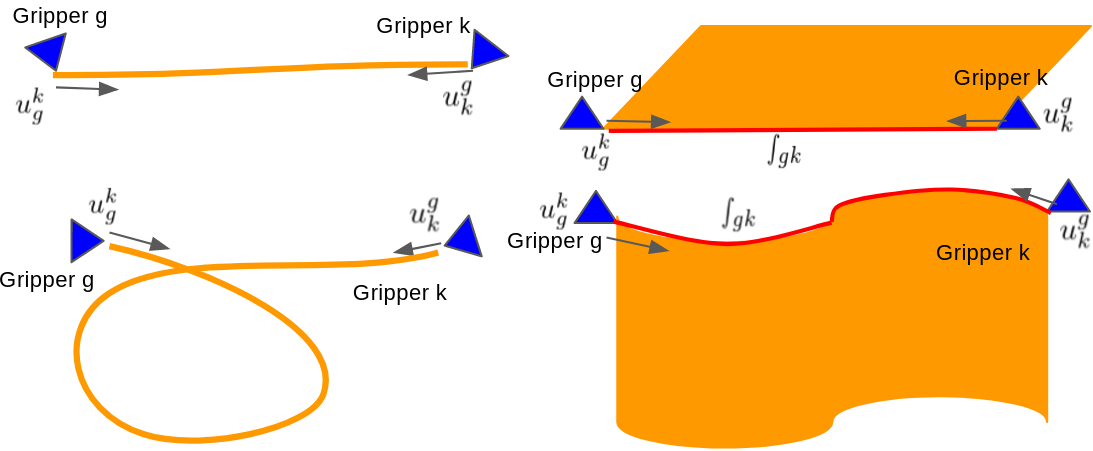
\includegraphics[width=.98\linewidth]{Stretching_vector_method.png}
  \caption{The arrows in gray show the direction of each stretching vector at the corresponding gripper with respect to the gripper pair $q_g$ and $q_k$. Left: stretching vectors on the rope when the rope is at rest (above) or is deformed (below). Right: stretching vectors on the cloth when the cloth is at rest (above) or is deformed (below). The red lines denote the geodesic connecting the corresponding $p_{\mathcal{I}_g(q_g,q_k)}$ and $p_{\mathcal{I}_k(q_g,q_k)}$ on the object.}
  \label{Fig: stretching_avoidance_vector_method}
\end{figure}
%\todo{Talk about the optimizer you use (Gurobi?)} 


\subsection{Optimization Method}

%\todo{have Dale confirm this section is correct}
Because our objective function is not necessarily convex, we used a custom optimization method to solve the problem specified in Eq. \ref{Eq: Optimization Problem}. Our method is a type of numerical gradient descent with an additional projection step to enforce constraints.

Our method's outer loop computes the numerical gradient of the objective function. An inner loop then performs backtracking line search to find the gradient step size. However, the gradient step may cross a constraint boundary, thus after we compute the step size, we check if any constraint has been violated after taking the step. If it has, we project the step back to the feasible space. A simple projection to the boundary of a violated constraint may satisfy that constraint but violate others. Instead, to perform the projection, we solve a convex optimization problem (using the Gurobi optimizer \cite{Gurobi2017}) to find the nearest feasible point. This is possible because all the constraints in our problem are convex. Once such a point is found, the outer loop continues to iterate until convergence.


%\textcolor{red}{In this paper, our main focuses are designing a more accurate model without the high cost and integrating the constraints on the controller and thus we didn't explore the more advanced optimization algorithm.
%Considering the highly non-linearity of the model, we use the numerical gradient descent to solve the Eq.\ref{Eq: Optimization Problem}}






%%%%%%%%%%%%%%%%%%%%%%%%%%%%%%%%%%% Results %%%%%%%%%%%%%%%%%%%%%%%%%%%%%%%%%%%%%%%%%%%%%%%%%%%%%%%%%


\section{RESULTS}


%\todo{1). Please give the quantified results of the accuracy 
%and computation cost, and explain why 'Our two goals are improving the accuracy of the deformable...'"; 
%2). Please explain how to set or tune all the parameters and ratios and show the influence of different parameters, ratios and time step;
%3). Please test the performance of the presented methods with different objects and tasks. And the results should be reported with quantified figures or tables.
%}




%\todo{make sure values for ALL parameters described in the methods section are specified in the results section}





%Our two goals are improving the accuracy of the deformable object manipulation controller and 
Our two goals are improving the accuracy of the deformable object motion model (for use in the controller), 
and formulating a set of constraints for the controller to mitigate collision and excessive stretching issues.
As mentioned in previous sections, our benchmark model and controller is \cite{Berenson2013}. To evaluate our method we perform experiments in simulation and on a physical robot. The simulator used is Bullet physics \cite{Coumans2010}, however, we emphasize that our method has no knowledge of the simulation parameters or simulation methods used therein. The simulator is used as a ``black-box,'' mainly to stand in for a perception system and to allow us to do repeatable experiments. The physical robot consists of two KUKA iiwa 7DoF arms with Robotiq 3-finger hands.


%, which would be difficult to construct in the physical world.

%We set up both simulation experiments and real-robot experiments. 
%We furthermore perform the quantitative analysis of the performance on the simulation ones. 
%In the following section, \ref{Results:Simulation and Quantitative Analysis} shows the results from simulation and \ref{Results:Real-robot Experiment} shows the ones from the real-robot experiment.



%\subsubsection{General Experimental Setup}
We ran experiments with scenarios involving both cloth and rope.
%We ran four experiments with two each for the 1D rope and the 2D cloth. 
%The four task-scenes are showed in Fig. \ref{Fig: experimental_setup_scene}, where grippers are to manipulate the rope or cloth to cover the red points. 
The parameters are set as $k_g = 4$, $k_D = 10$, $k_{r} = 20$ 
%\todo{"should it be $k_r$ mentioned in previous sections?"} 
for the new model, $l_c = 0.023$, and $s_s = 0.4$ for the new controller. 
The parameters we used for the benchmark method are its default best value found in \cite{McConachie2018}. The stretching detection ratio is set as $\gamma_s = 1.667$ for the cloth and $\gamma_s = 1.1$ for the rope.
The maximum gripper motion is set as $\Delta_{q,\textrm{max}} = 0.03$, with time step $\Delta t = 0.01$s.
For the experiment with a task goal defined, a precalculated Dijkstra field for the task will generate the $\Delta \mathcal{P}_d$ for each point at each state to move the object toward the goal given each point's current position in the space. All experiments were run on a i7-8700K 3.7 GHz CPU with 32 GB of RAM. A video showing the experiments is included with this paper.

\subsection{Model Accuracy Results} \label{Results:accuracy}

%As a result, 
%the $\Delta\mathcal{P}_d$ generated could be an unachievable motion so that there is an intrinsic control error. 
%To eliminate the effects from this intrinsic control error so as to make the control errors easier to be compared, we used relative error $e^r$ instead of comparing $e$ directly, where $e^r_o = e_o - \textrm{min} \{e_o, e_n \}$ for the benchmark, and $e^r_n = e_n - \textrm{min}\{e_o, e_n \}$ for the new controller.



We evaluated model accuracy by pulling the rope in a straight line along the direction of the rope, then turning the gripper and pulling back towards the rope as shown in Fig.~\ref{Fig: intro_Directional_rigidity}. As shown in Fig.~\ref{Fig: rope_model_accuracy_plot}, our new model is a better approximation of the true motion when the gripper is pulling the rope. When the gripper is turning, both the baseline and the new model produce comparable error, but when the gripper starts pulling again (this time in the opposite direction), the new model is a significantly better approximation.

We also evaluated model accuracy by pulling the cloth in a similar fashion; pulling the cloth one way, turning the grippers, and then pulling in the opposite direction. As shown in Fig.~\ref{Fig: cloth_model_accuracy_plot}, our new model is a better approximation of the true motion when the grippers are pulling the cloth. As in the rope test, when rotating the grippers both models produce comparable error. While the cloth is folded on itself both models produce noisy results, but when the cloth lies flat again, the new model achieves lower error.

\begin{figure}[t]
    \centering
    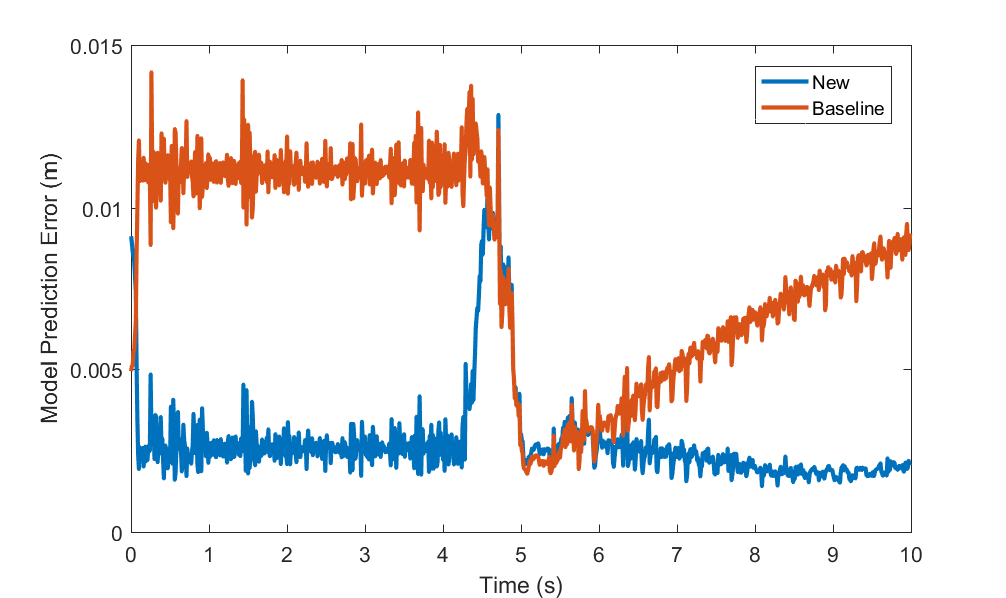
\includegraphics[width=\columnwidth]{rope_model_accuracies.png}
    \caption{RMS model prediction error. The gripper pulls the rope for the first 4.5 seconds, then turns for half a second, then moves in the opposite direction at the 5 second mark.}
    \label{Fig: rope_model_accuracy_plot}
\end{figure}

\begin{figure}[t]
    \centering
    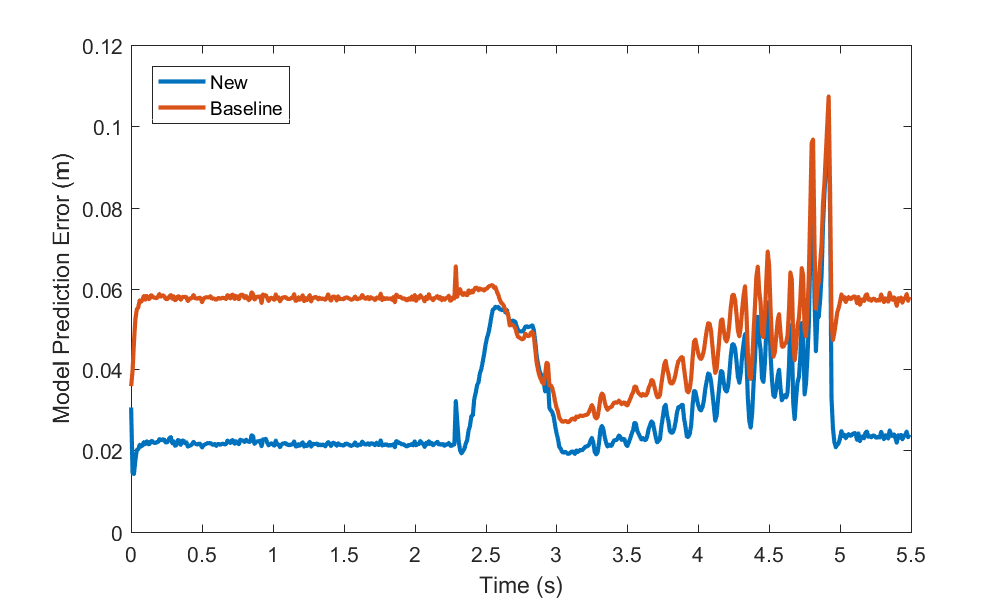
\includegraphics[width=\columnwidth]{cloth_model_accuracies.png}
    \caption{RMS model prediction error. The grippers pull the cloth for the first 2.3 seconds, then turn for 0.63 seconds, then move in the opposite direction at the 2.93 second mark. At the 5 second mark the cloth is no longer folded. }
    \label{Fig: cloth_model_accuracy_plot}
\end{figure}









%In this section, we show the model prediction performance in \ref{Results:Model Accuracy}, controller stretching avoidance performance in \ref{Results: Object Stretching Avoidance}, and controller task achieving performance in \ref{Results:Controller Task Performance}. Fig.\ref{Fig: experimental_setup_scene} shows the scenes of the setups. 


\subsection{Constraint Enforcement}
\label{Results: Object Stretching Avoidance}

Since the benchmark controller can already handle the collision constraint very well, and the new controller addresses the collision constraint in the similar way as the benchmark, there is not a significant difference in how the collision constraint is enforced. However, the stretching constraint shows a very clear improvement.

The metrics of stretching avoidance is the stretching ratio $\gamma$ defined in Section \ref{Method_Overstretch}. A controller with good stretching avoidance should prevent $\gamma$ from increasing beyong a certain threshold.

The two experiments we used for the stretching avoidance test are the rope-wrapping-cylinder and the cloth-passing-single-pole, shown in Fig.\ref{Fig: scene_1_rope_zig_match} and Fig.\ref{Fig: scene_4_cloth_single_pole}. 
We ran each controller separately for a fixed amount of time for each task and show $\gamma$ vs. time for both controllers in Fig. \ref{Fig: experiment_stretching_factor} . 
In both these two setups, the desired object motion $\dot{\mathcal{P}}_d$ generated by the Dijkstra field will tear the object unless overstretching is prevented.%, thus the $\gamma$ will keep going up without good stretching correction from the controller.

Fig. \ref{Fig: experiment_stretching_factor} shows the new controller is able to prevent further stretching happening when the object is taut for both the rope and the cloth. 
In the rope test, the new controller can prevent overstretching with $s_s = 0.4$, as defined in Eq.\ref{Eq: Stretching_avoidance_Method_This_Paper}. 
We can see the $\gamma$ of the benchmark methods keeps growing beyond this threshold, while the $\gamma$ of the new method stays close to the threshold. In the cloth test, the benchmark method's $\gamma$ (in purple) increases above the threshold $\gamma_s = 1.667$ for cloth, and a sudden drop in $\gamma$ happens after running the test for $2$ seconds. This drop is the ``tearing'' point in the simulator. Though we still see overstretching happened using the new method for some settings of $s_s$, in all cases the $\gamma$ converged before tearing happened (instead of growing without bound). 
%Moreover, the overstretching was reduced with a tighter constraint set by increasing the $s_s$. 

\begin{figure}[t]
\begin{subfigure}{.24\textwidth}
  \centering
  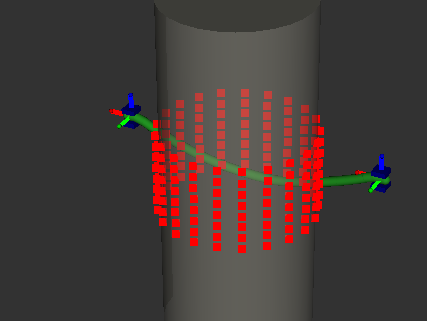
\includegraphics[width=.9\linewidth]{rope_cylinder}
  \caption{Rope wrapping cylinder}
  \label{Fig: scene_1_rope_zig_match}
\end{subfigure}%
\vspace{0.3cm}
\begin{subfigure}{.24\textwidth}
  \centering
  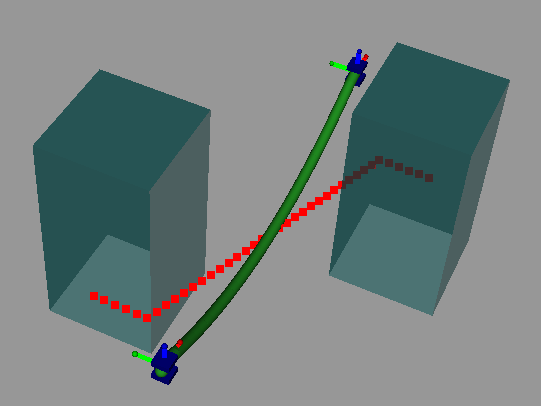
\includegraphics[width=.9\linewidth]{rope_zig_match}
  \caption{Rope matching zig-path}
  \label{Fig: scene_2_rope_zigzag}
\end{subfigure}
\begin{subfigure}{.24\textwidth}
  \centering
  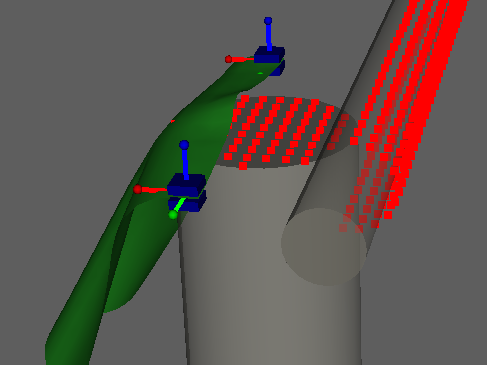
\includegraphics[width=.9\linewidth]{cloth_wafr}
  \caption{Cloth covering two cylinders}
  \label{Fig: scene_3_cloth_wafr}
\end{subfigure}
\begin{subfigure}{.24\textwidth}
  \centering
  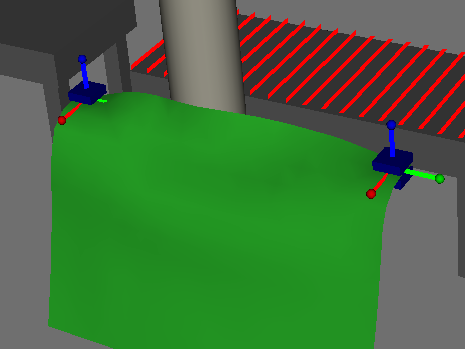
\includegraphics[width=.9\linewidth]{cloth_single_pole}
  \caption{Cloth passing single pole}
  \label{Fig: scene_4_cloth_single_pole}
\end{subfigure}
\caption{Initial state of the four experiments, where the red points act as attractors for the deformable object.}
\label{Fig: experimental_setup_scene}
\end{figure}










\begin{figure}[t]
\begin{subfigure}{.24\textwidth}
  \centering
  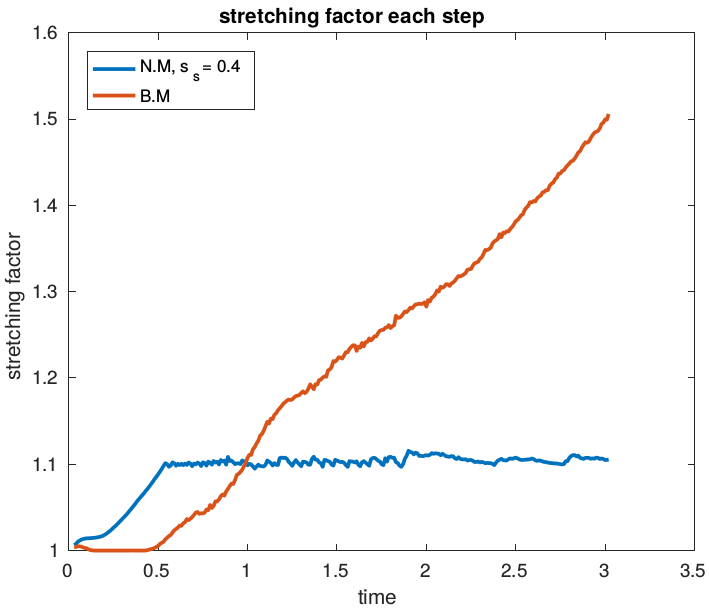
\includegraphics[width=.99\linewidth]{stretching_rope_cylinder}
  \caption{Rope wrapping cylinder}
  \label{Fig: stretching factor scene_rope_cylinder}
\end{subfigure}
\begin{subfigure}{.24\textwidth}
  \centering
  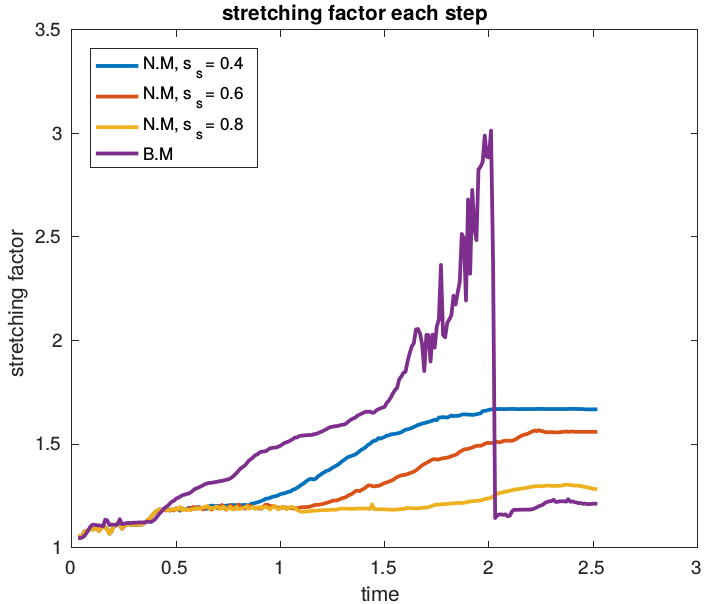
\includegraphics[width=.99\linewidth]{stretching_cloth_single_pole}
  \caption{Cloth passing single pole}
  \label{Fig: stretching factor scene_cloth_single_pole}
\end{subfigure}
\caption{(a) The red line shows the $\gamma$ of the benchmark and the blue line shows the $\gamma$ of the new controller with $s_s = 0.4$ throughout the simulation. (b) The purple line shows the $\gamma$ of the benchmark, and the blue, red, and yellow lines each show the $\gamma$ of the new controller with $s_s = 0.4$, $s_s = 0.6$, and $s_s = 0.8$, respectively.}
\label{Fig: experiment_stretching_factor}
\end{figure}




%We find that setting a tighter constraint, such as increasing the value of $s_s$, can help prevent excessive stretching in the object, as shown in Fig. \ref{Fig: cos_stretching}. 


% Explain the trade-off between constraints avoidance and control accuracy
%Examining Fig. \ref{Fig: experiment_model_error} and Fig. \ref{Fig: experiment_stretching_factor}, we found that when there is no constraints violation detected, the new controller can generally have a smaller control error.
%When the constraints violation happens, the new controller will tend to mitigate this violation and take the trade off in control accuracy.  



\subsection{Controller Task Performance} \label{Results:Controller Task Performance}

Besides the quantitative analysis of the model accuracy and stretching avoidance, we ran another two experiments, rope-matching-zig-path and cloth-covering-two-cylinder, one each with the rope or the cloth, as shown in Fig.\ref{Fig: scene_2_rope_zigzag} and Fig.\ref{Fig: scene_3_cloth_wafr} to see how the new method performed for some coverage tasks. Both the benchmark and the new controllers are able to perform these tasks with comparable performance; reaching approximately the same configurations when forward progress stops due to a local minimum (Fig.~\ref{Fig: cloth_wafr_performance}), and completing the task (Fig.~\ref{Fig: zigzeg_performance}). This result suggests that we have not lost functionality with respect to the benchmark despite changing the model and control method used.


\begin{figure}[ht!]
    \centering
    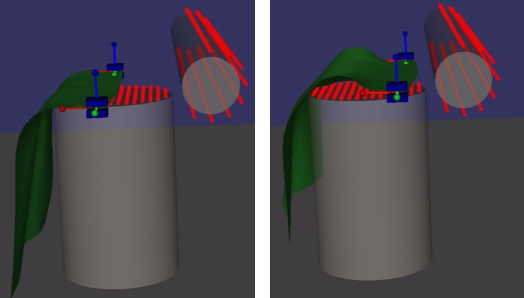
\includegraphics[width=\columnwidth]{cloth_wafr_performance.png}
    \caption{Cloth-covering-two-cylinder task start and end configurations. Both controllers are unable to make progress due to a local minima.}
    \label{Fig: cloth_wafr_performance}
\end{figure}


\begin{figure}[ht!]
    \centering
    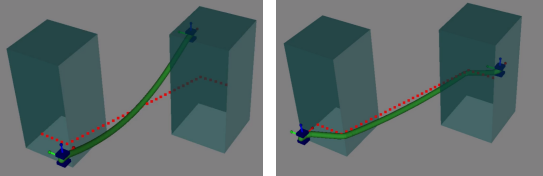
\includegraphics[width=\columnwidth]{zigzeg_performance.png}
    \caption{Rope-matching-zig-path start and end configurations. Both controllers are able to succeed at the task, bringing the rope into alignment with the desired path.}
    \label{Fig: zigzeg_performance}
\end{figure}



\subsection{Physical Robot Experiments}

To evaluate our new model and controller on a physical system, we set up two experiments with cloth-like objects manipulated by two 7DoF KUKA iiwa arms (Fig.~\ref{Fig: physical_experiment_screenshots}). To sense the position of the cloth, we use the AprilTags~\cite{olson2011tags} and IAI Kinect2~\cite{iai_kinect2} libraries. The parameters are set as $k_g = 4$, $k_D = 10$, $k_{r} = 10$ for the new model, $l_c = 0.08$, and $s_s = 0.6$ for the new controller. The first test, which evaluates model accuracy, uses a motion profile similar to the simulation accuracy tests (Fig.~\ref{Fig: cloth_model_accuracies_live}). Similar to the simulation results, the new model improves performance when dragging the cloth (first and last sections of Fig.~\ref{Fig: cloth_model_accuracies_live}), and is comparable during rotational motion and when the cloth is resting on edge perpendicular to the table (see video). To test the controller, we set up a task similar to the cloth-passing-single-pole example using a paper towel. For this task, the baseline controller tears the paper towel while the new controller avoids excessive overstretch, instead wrapping around the pole to reach a local minimum.

\begin{figure}[t]
    \centering
    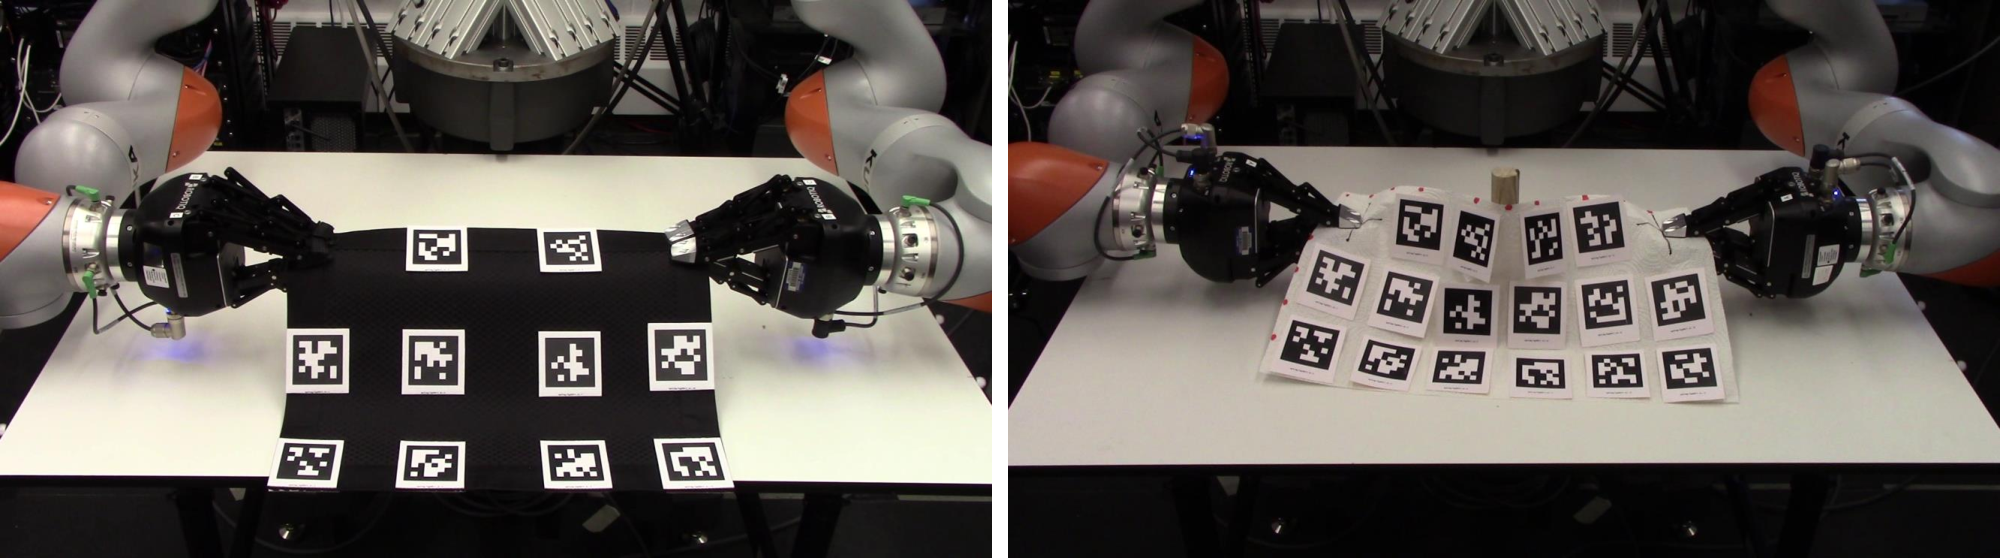
\includegraphics[width=\columnwidth]{physical_robot_experiment_screenshots.pdf}
    \caption{Initial setup for the physical robot experiments. Left: model accuracy test. Right: stretching avoidance test.}
    \label{Fig: physical_experiment_screenshots}
\end{figure}


\begin{figure}[t]
    \centering
    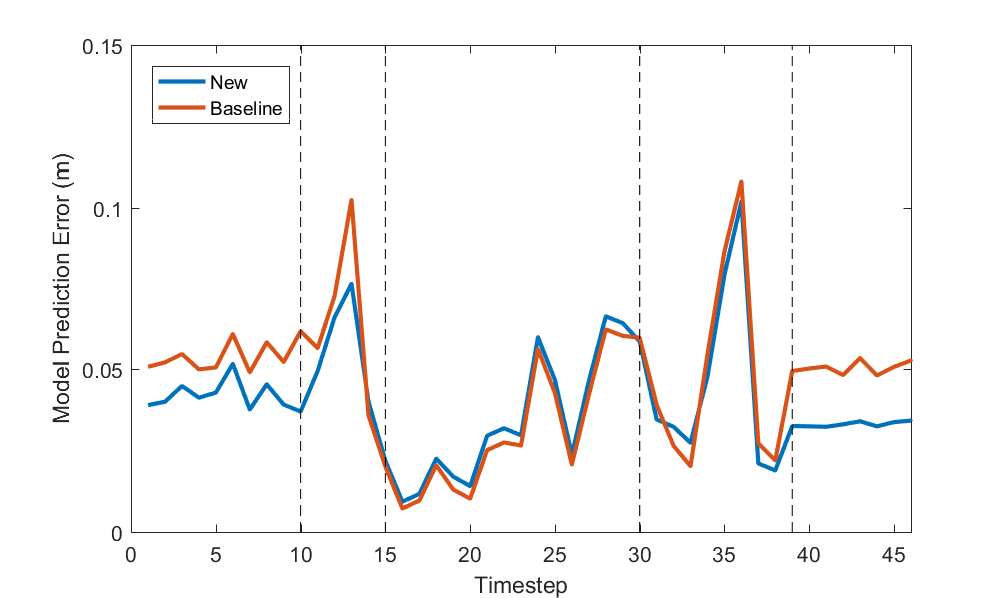
\includegraphics[width=\columnwidth]{cloth_model_accuracies_live.png}
    \caption{RMS model prediction error. The grippers pull the cloth toward the robot for the first 10 timesteps, upward for 5 timesteps, rotate for 15 timesteps, diagonally down and away for 9 timesteps, then directly away from the robot.}
    \label{Fig: cloth_model_accuracies_live}
\end{figure}



\subsection{Computation Time}


\begin{table}[t]
%\renewcommand{\arraystretch}{1.2}
\centering
\resizebox{\linewidth}{!}{
\begin{tabular}{|c|c|c|c|c|}
\hline
           & rope-wrapping & rope-matching & cloth-passing & cloth-wrapping \\
           & -cylinder     & -zig-path     & single-pole   & -two-cylinders \\
\hline
BM       & 0.0055   & 0.0054  & 0.0153  & 0.0037   \\
\hline
NM       & 0.0342   & 0.0834  & 0.2363  & 0.1008   \\
\hline
\end{tabular}
}
\caption{Mean computation time (s) to compute the gripper motion for a given state. BM: benchmark method; NM: new method.}
\label{Tbl: controller time report}
\end{table}

\begin{table}[t]
%\renewcommand{\arraystretch}{1.2}
\centering
\resizebox{\linewidth}{!}{
\begin{tabular}{|c|c|c|c|c|}
\hline
            & rope-wrapping & rope-matching & cloth-passing & cloth-wrapping \\
            & -cylinder     & -zig-path     & single-pole   & -two-cylinders \\
\hline
BT    & 0.686   & 0.571   & 19.29   & 3.680   \\
\hline
NM   & 0.029   & 0.014   & 1.172   & 0.339   \\
\hline
\hline
\# evals &  50.72 & 143.5 & 83.81 & 63.32\\
% \hline
% \rev{T.C}   & \rev{1.473}   & \rev{4.810}   & \rev{98.240}  & \rev{21.135}  \\
\hline
\end{tabular}
}
\caption{Top two rows: Mean computation time (ms) per model prediction for a given gripper motion. BT: Bullet simulator; NM: new model. Bottom row: Mean number of times the model was evaluated when executing the new method.}%; T.C: total model computation time per controller iteration.}}
\label{Tbl: simulation time report}
\end{table}



To verify the practicality of our method, we gathered data comparing its computation time to the benchmark's and to using the Bullet simulator. Table~\ref{Tbl: controller time report} shows the average computation time of a call to the controller for the new method vs. the benchmark. As expected, the benchmark, which uses a linear model, is faster than the new method. However, the computation times for the new method are still reasonable to use in a control loop.

Table~\ref{Tbl: simulation time report} shows a comparison between the average time needed to evaluate the new model and the time needed to simulate a gripper motion with the Bullet simulator. Note that the amount of time required for the simulator to converge to a stable estimate depends on many conditions, including what object is being simulated. Through experimentation we determined that 4 simulation steps were adequate for rope and 10 for cloth. Comparing the time needed to do this simulation to the time needed to evaluate our model, we see that the new model is indeed faster by at least an order of magnitude, in some cases by two orders of magnitude, confirming that, despite being slower than the benchmark, our method still outperforms the simulator in terms of computation time.























%\subsection{Real-robot Experiment} \label{Results:Real-robot Experiment}


%Besides the experiments run with the simulator, we also tested the quality of the controller on the real-robot. 





\section{CONCLUSION}
%\todo{"the author claims that “thus maintaining low computation cost”. Please give the quantified results (considering 1D/2D/3D objects and including the off-line process) and explain why."}

In this paper we extended a geometric model for deformable object manipulation to include directional rigidity and obstacle penetration constraints. Considering these terms in the model allowed us to improve the model's prediction while maintaining low computation cost. We also addressed the excessive stretching issue by approximating the stretching constraints with conical constraints around stretching avoidance vectors. Our controller is able to complete the same tasks as the previous benchmark method but also correctly enforces stretching constraints when the object is caught on obstacles. In future work, we would like to investigate the sensitivity of the model with respect to its parameters and develop methods to automatically tune these parameters based on observed motion.